
Pour mesurer les précipitations, Météo France utilise deux sortes
de pluviomètres:

\begin{itemize}
\item des pluviomètres à lecture directe ;
\item des pluviomètres électroniques.
 \end{itemize}
 
La mesure des précipitations s'exprime en millimètre. On donne ainsi la hauteur d'eau $H$
qui est tombée en utilisant la formule :
\begin{center}
\begin{tabularx}{\linewidth}{m{2.5cm}X }
$H = \dfrac{V}{S}$&
où $V$ est le volume d'eau tombée sur une surface $S$.

Pour $H$ exprimée en mm, $V$ est exprimé en mm$^3$ et $S$ en mm$^2$.
\end{tabularx}
\end{center}

\medskip

\textbf{Partie I : Pluviomètres à lecture directe}

\medskip

Ces pluviomètres sont composés d'un cylindre de réception et d'un réservoir conique
gradué.

\medskip

\begin{enumerate}
\item Vérifier à l'aide de la formule que lorsqu'il est tombé $1$~mm de pluie, cela correspond
à 1~L d'eau tombée sur une surface de 1 m$^2$.
\item Un pluviomètre indique $10$~mm de pluie. La surface qui reçoit la pluie est de $0,01$~m$^2$.

Quel est le volume d'eau dans ce pluviomètre ?
\end{enumerate}

\medskip

\textbf{Partie II : Pluviomètres électroniques}

\medskip

Durant un épisode pluvieux, on a obtenu le graphique suivant grâce à un pluviomètre
électronique :

\begin{center}

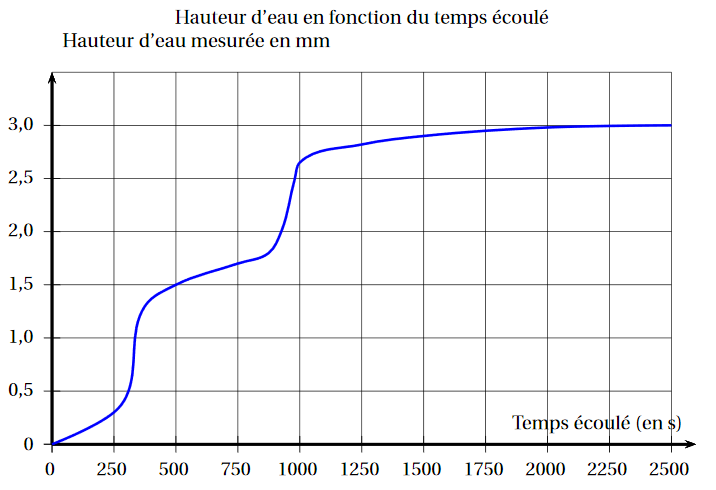
\includegraphics[scale=1]{NF-46.png} 

\end{center}

\begin{enumerate}
\item L'épisode pluvieux a commencé à 17~h~15.

Vers quelle heure la pluie s'est-elle arrêtée ?
\item On qualifie les différents épisodes pluvieux de la façon suivante :

\begin{center}
\begin{tabularx}{\linewidth}{|*{2}{>{\centering \arraybackslash}X|}}\hline
\textbf{Types de pluie}	& \textbf{Vitesse d'accumulation}\\ \hline
Pluie faible 			&Jusqu'à 2,5~mm/h\\ \hline
Pluie modérée 			&Entre 2,6 à 7,5~mm/h\\ \hline
Pluie forte 			&Supérieure à 7,5~mm/h\\ \hline
\end{tabularx}
\end{center}

À l'aide des informations données par le graphique et le tableau ci-dessus, cette pluie
serait-elle qualifiée de faible, modérée ou forte ?
\end{enumerate}